\documentclass[10pt,a4paper]{report}
\usepackage[utf8]{inputenc}
\usepackage[czech]{babel}
\usepackage[T1]{fontenc}
\usepackage{amsmath}
\usepackage{amsfonts}
\usepackage{mwe}
\usepackage{amssymb}
\usepackage{graphicx}
\usepackage{subcaption}
\author{Pavla Kratochvílová, Adriana Šmijáková}
\title{IV109 - Formace názorů}

\begin{document}
\maketitle
% stručné uvedení do tématu, objasnění základních pojmů
\chapter{Úvod}
Naším cílem je zachytit proces formování názorů, který probíhá při interakcích lidí v sociální síti. Vycházíme z myšlenky, že názory člověka jsou do značné míry ovlivněny názory v jeho okolí. Uvažujeme přitom spojitý názor -- člověk nemusí pouze zcela přijmout nebo zamítnout názor svého okolí, ale může jen lehce poupravit svůj vlastní názor tak, aby se více přiblížil názoru okolí. 

Formování názorů zkoumáme s různým počátečním rozložením názorů a na několika typech sítí: náhodný graf, prostorový graf, malý svět a preferenční graf. Ačkoliv se neumíme zcela přiblížit reálným komplexním sítím, vybrané grafy mají některé vhodné vlastnosti, které nalezneme i u komplexních sítích. 

Náhodný graf a malý svět mají oproti ostatním grafům poměrně malé průměrné vzdálenosti mezi vrcholy. Prostorový graf a malý svět zase vykazují poměrně vysoký stupeň shlukování. Preferenční graf jsme zařadily pro jeho distribuci stupňů vrcholů, která se řídí mocninným zákonem.

\chapter{Návrh modelu}
Formování názorů modelujeme pomocí agentů, kdy každý agent má přidělen názor vyjádřený reálným číslem z intervalu $\langle 0, 1 \rangle$. Agenti jsou vzájemně propojeni v rámci určitého grafu a interagují spolu pouze agenti spojení vazbou.

Model se skládá ze dvou částí: nejprve se vytvoří síť agentů a každému se nastaví názor, a poté probíhá samotný proces formování názorů.

\section{Tvorba grafu}
Všechny grafy jsou parametrizovány počtem vrcholů (parametr \texttt{people}) a prů\-měr\-ným stupněm vrcholů (parametr \texttt{average-node-degree}). Uvažovali jsme čtyři různé typy grafů:

\begin{itemize}
	\item Náhodný graf vzniká náhodným přidáváním hran, dokud neodpovídá prů\-měr\-ný stupeň vrcholů.
	\item Prostorový graf (spatial graph) je převzatý z již existujícího modelu \textit{Virus on a Network}. Je vytvořen náhodným rozmístěním agentů do prostoru a následným přidáváním hran, dokud neodpovídá průměrný stupeň vrcholů. Hrany jsou přidávány mezi náhodným agentem a jemu nejbližším agentem, se kterým ještě není spojen.
	\item Malý svět je založený na existujícím modelu \textit{Small World}. Nejprve je vytvořen cyklus všech agentů, a poté jsou přidány hrany mezi agenty vzájemně vzdálenými méně než nějaké n tak, aby se stupeň vrcholu co nejvíce přiblížil zvolenému průměrnému stupni. Následně některé hrany zamění jeden svůj konec za náhodný jiný. Počet takových hran je dán nepřímo parametrem \texttt{rewiring-prob}.
	\item Preferenční graf je založený na existujícím modelu \textit{Prefferential Attachment}. Vzniká postupným přidáváním vrcholů, přičemž nový vrchol se spojí s nějakým již existujícím. Upřednostňovány jsou vrcholy, které mají více hran -- toho je dosaženo náhodným výběrem z konců hran raději než výběrem z vrcholů. V preferenčním grafu se parametr \texttt{average\--node\--degree} nebere v úvahu.
\end{itemize}

Výběr typu grafu lze provést pomocí parametru \texttt{network-type}.

\section{Počáteční rozložení názorů}
Agentům jsou přiřazeny názory v intervalu $\langle 0, 1 \rangle$. Uvažovali jsme tři možná počáteční rozložení názorů:

\begin{itemize}
	\item Uniformní rozložení.
	\item Normální rozložení -- s průměrem $0.5$ a standardní odchylkou $0.2$.
	\item Normální rozložení se středem v extrémech -- stejné jako normální rozložení v předchozím bodě, ale posunuté tak, aby nejvíce názorů bylo extrémních (tj. těsně nad $0$ a těsně pod $1$) a nejméně středových (tj. okolo $0.5$).
\end{itemize}

Počáteční rozložení názorů lze změnit pomocí parametru \texttt{opinion-distri\-bution}. 

\section{Změny názorů}
Uvažujeme dvě strategie pro změnu názorů:

\begin{itemize}
	\item Jeden soused -- agent se podívá na jednoho náhodného agenta ze svého okolí a podle jeho názoru změní svůj vlastní názor.
	\item Všichni sousedé -- agent se podívá na všechny agenty ve svém okolí a podle jejich průměrného názoru změní svůj vlastní názor.
\end{itemize}

V obou případech proběhne změna názoru stejným způsobem. Agent nejprve vypočte rozdíl mezi svým názorem a názorem okolí (tj. buď názor vybraného souseda, nebo průměrný názor všech sousedů), a následně posune svůj názor o zlomek tohoto rozdílu směrem k názoru okolí. Velikost zlomku je daná parametrem \texttt{changing-opinion-strength} (síla změny názoru).








\chapter{Simulace a analýza}
Model formování názorů jsme navrhly tak, že se agenti svými názory neustále přibližují svému okolí. Jestliže je tedy graf spojitý, názory konvergují k nějaké hodnotě, v našem případě v okolí $0.5$. Z toho důvodu jsme se spíše než na výsledek dlouhodobého běhu simulace zaměřily na průběh samotného formování názorů.

Při analýze pracujeme s grafy fixní velikosti: počet lidí je 100; průměrný stupeň vrcholů (s výjimkou preferenčního grafu) je 7; a pravděpodobnost předrátování $30\thinspace\%$, díky čemuž má graf malý svět podobnou průměrnou délku nej\-kratších cest jako preferenční graf.

V některých případech je třeba zafixovat hodnoty parametrů, na které se právě nezaměřujeme. V takových případech je hodnota parametru \texttt{changing\--opinion\--strength} $0.1$, počáteční rozložení názorů je uniformní a strategie pro změnu názorů je jeden soused.

\section{Množství změn}
V této sekci jsou rozebrány vlivy jednotlivých parametrů na množství změn názorů v čase. Množství změn (v diagramech \texttt{changes}) je určeno jako součet změn všech názorů agentů, které proběhnou v daném časovém okamžiku, a dobře tak odráží celkovou dynamiku modelu.

Všechny diagramy, které zachycují množství změn názorů, vznikly zprů\-mě\-ro\-vá\-ním deseti běhů se stejně nastavenými parametry.

\subsection{Síla změny názoru}
Nejprve chceme ukázat vliv parametru \texttt{changing-opinion-strength} na množ\-ství změn názorů v čase. Vzhledem k tomu, že jsou velikosti změn názorů ovlivněné samotnou hodnotou parametru \texttt{changing-opinion-strength}, obrá\-zek \ref{fig:zmeny-nenormovany-normovany} zobrazuje jak diagram s původními hodnotami změn, tak i diagram s~normovanými hodnotami. 

\begin{figure}[h]
\begin{subfigure}{.5\textwidth}
  \centering
  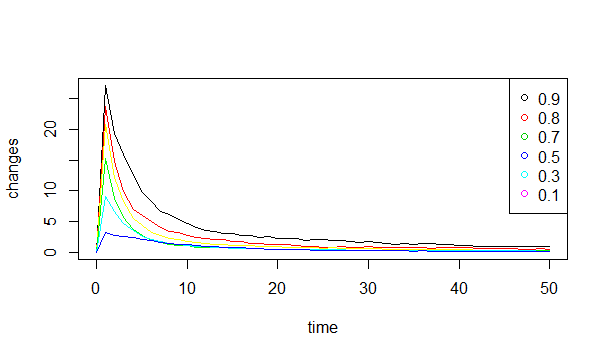
\includegraphics[width=1\linewidth]{plots/spatial-g/spatialChanges1-9.png}
  \caption{Nenormovaný diagram}
  \label{fig:zmeny-nenormovany}
\end{subfigure}%
\begin{subfigure}{.5\textwidth}
  \centering
  
  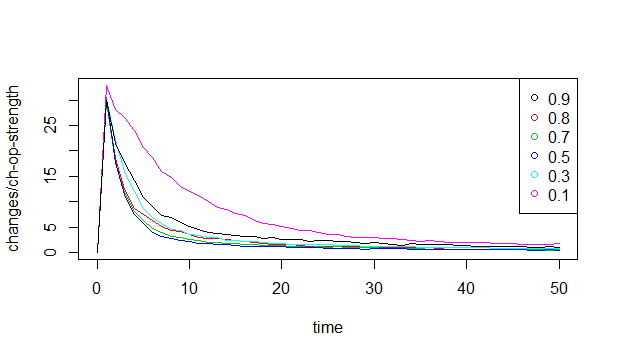
\includegraphics[width=1\linewidth]{plots/spatial-g/spatialChanges1-9norm.png}
  \caption{Normovaný diagram}
  \label{fig:zmeny-normovany}
\end{subfigure}
\caption{Prostorový graf -- vývin množství změn vlivem parametru \texttt{changing-opinion-strength}}
\label{fig:zmeny-nenormovany-normovany}
\end{figure}

Je zde ukázáno, že nejrychleji se názor ustálí při síle změny názoru $0.5$. Čím více se však síla změny názoru blíží k $0$ nebo $1$, tím déle trvá ustálení názoru. Nejvýraznější by byl případ parametru s hodnotou $1$, ale tato situace je velice specifická -- agenti neupravují svůj názor jen částečně, ale názor okolí (podle vybrané strategie) zcela přeberou -- a proto ji do analýzy mimo parametr \texttt{changing-opinion-strength} nezahrnujeme. Hodnota $1$ je zároveň jediná, u které je možné sledovat konvergenci názorů i k~hodnotě vzdálené od $0.5$.

V normovaném diagramu je množství změn výraznější pro extrémnější hodnoty síly změny názoru (tj. bližší k $0$ nebo $1$) a konvergence trvá déle. Pokud potom porovnáme hodnoty stejně vzdálené od $0.5$, výraznější změny jsou u hodnot menších než $0.5$. 

Na obrázku \ref{fig:zmeny-grafy} vidíme porovnání vlivu \texttt{changing-opinion-strength} pro různé typy grafů.

\begin{figure*}[h]
  \centering
  \begin{subfigure}[b]{0.475\textwidth}
      \centering
      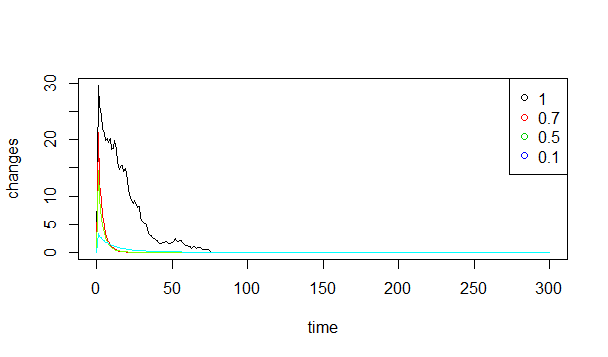
\includegraphics[width=\textwidth]{plots/random-g/changesRandom.png}
      \caption[Network2]%
      {{\small Náhodný graf}}    
      \label{fig:zmeny-nahodny}
  \end{subfigure}
  \hfill
 \begin{subfigure}[b]{0.475\textwidth}   
      \centering 
      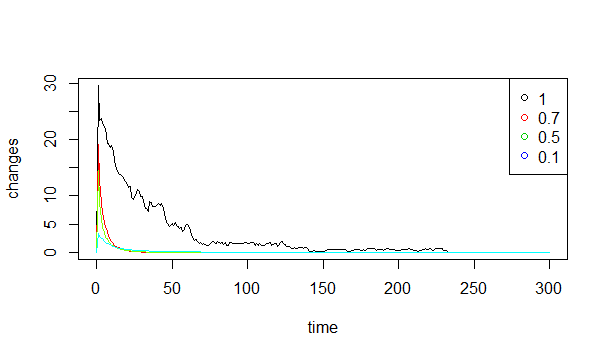
\includegraphics[width=\textwidth]{plots/small-world-g/changesSmallWorld.png}
      \caption[]%
      {{\small Prostorový graf}}    
      \label{fig:zmeny-prostorovy}
  \end{subfigure}
  \vskip\baselineskip
  
    \begin{subfigure}[b]{0.475\textwidth}  
      \centering 
      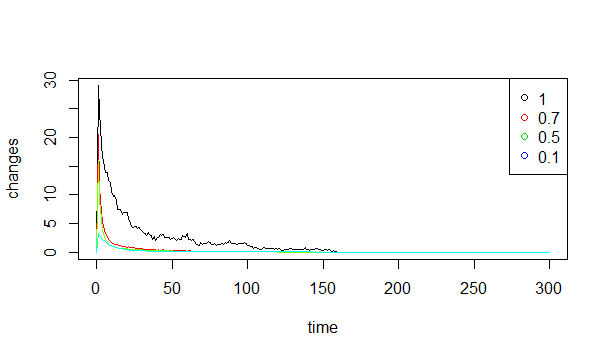
\includegraphics[width=\textwidth]{plots/spatial-g/ChangesOneSpatial.png}
      \caption[]%
      {{\small Malý svět}}    
      \label{fig:zmeny-maly svet}
  \end{subfigure}
  \quad
  \begin{subfigure}[b]{0.475\textwidth}   
      \centering 
      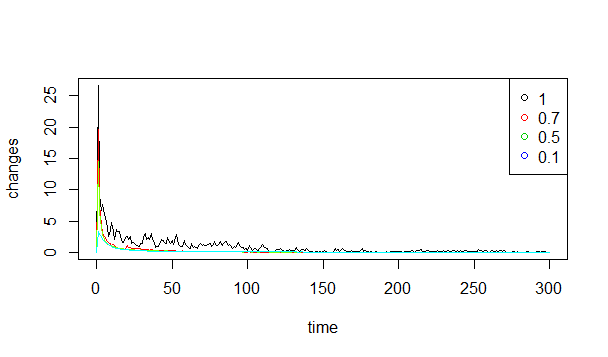
\includegraphics[width=\textwidth]{plots/prefferential-g/changesPrefferential.png}
      \caption[]%
      {{\small Preferenční graf}}    
      \label{fig:zmeny-preferencni}
  \end{subfigure}
  \caption[]
  {\small Vývin množství změn pro jednotlivé grafy vlivem parametru \texttt{changing-opinion-strength}}
  \label{fig:zmeny-grafy}
\end{figure*}

Když porovnáme různé grafy, pozorujeme pouze malé rozdíly pro hodnoty $\texttt{changing-opinion-strength} < 1$. Pokud se však zaměříme na hodnotu $1$, vyniknou zejména preferenční a náhodný graf. V preferenčním grafu se velmi rychle názory rozšíří a následně už jen malý počet agentů mění názory v porovnání s~jinou topologií. Prostorový graf je těmito vlastnostmi podobný, ale o něco méně výrazný. V náhodném grafu se agenti zase nejrychleji shodnou a dále se stav nemění.

\subsection{Počáteční rozložení názorů}
Diagram \ref{fig:zmeny-rozlozeni}, vytvořený nad náhodným grafem, ukazuje vliv počátečního rozložení názorů na množství změn. Rozložení \texttt{middle} zde označuje normální rozložení s průměrem $0.5$ a standardní odchylkou $0.2$, \texttt{extremes} označuje stejné rozložení, ale posunuté tak, aby nejvíce názorů bylo extrémních (tj. těsně nad $0$ a těsně pod $1$) a nejméně středových (tj. okolo $0.5$). 

Normální rozložení má oproti ostatním větší dopad na vývin množství změn názorů. Vzhledem k tomu, že názory lidí v našem modelu konvergují k hodnotě $0.5$, toto rozložení konvergenci výrazně urychlí.

\begin{figure}[h]
  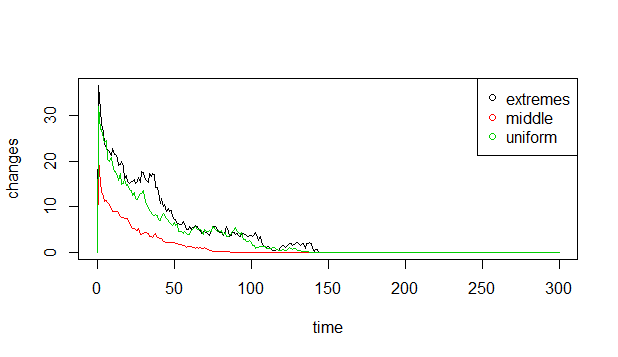
\includegraphics[width=\textwidth]{plots/small-world-g/smallWorldDistribution.png}
  \caption{Vývin množství změn vlivem parametru \texttt{opinion-distribution}}
  \label{fig:zmeny-rozlozeni}
\end{figure}

\subsection{Strategie změny názoru}
Podobně jako počáteční normální rozložení názorů, strategie zohledňující všechny sousedy urychluje ustálení jednotného názoru. Tento trend ukazuje diagram \ref{fig:zmeny-strategie}, který byl vytvořen nad prostorovým grafem.

\begin{figure}[h]
  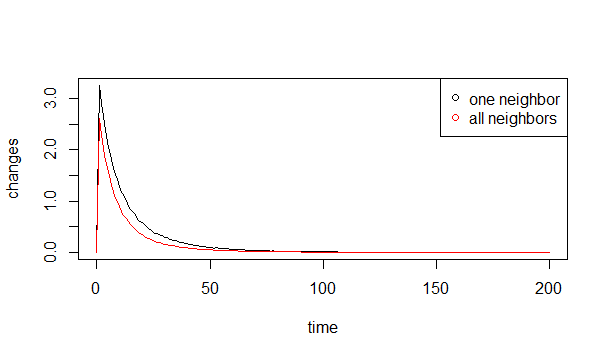
\includegraphics[width=\textwidth]{plots/random-g/randomAllVsOne.png}
  \caption{Vývin množství změn vlivem parametru \texttt{changing-opinion-strategy}}
  \label{fig:zmeny-strategie}
\end{figure}

\section{Průběh formování názorů na různých grafech}
Změny chování modelu pro různé topologie ukazoval už obrázek \ref{fig:zmeny-nenormovany-normovany}, avšak nevypovídal o konkrétních hodnotách názorů. Průběh změn hodnot můžeme vidět na obrázku \ref{fig:prubeh-grafy}. Znázorňuje názory nacházející se v určitém percentuálním umístění ve spektru hodnot od nejnižší (0\thinspace\%) po nejvyšší (100\thinspace\%). Střední hodnota má v diagramech hodnotu 50\thinspace\%. Oproti předchozím tyto diagramy nevznikly zprůměrováním hodnot z více běhů, ale znázorňují jen průběh jednoho běhu. Navzdory tomu je vzorek reprezentativní i pro opakovaný běh.

Pozorujeme podobné vlastnosti grafů jako v případě obrázku \ref{fig:zmeny-nenormovany-normovany}. V náhodném grafu a v malém světě názory velmi rychle konvergují a dále zůstávají neměnné.

\begin{figure*}[h]
  \centering
  \begin{subfigure}[b]{0.475\textwidth}
      \centering
      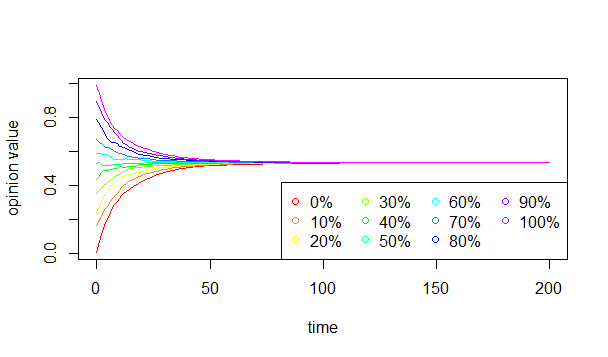
\includegraphics[width=\textwidth]{plots/max-values/random-maxv.png}
      \caption[Network2]%
      {{\small Náhodný graf}}    
      \label{fig:prubeh-nahodny}
  \end{subfigure}
  \hfill
  \begin{subfigure}[b]{0.475\textwidth}  
      \centering 
      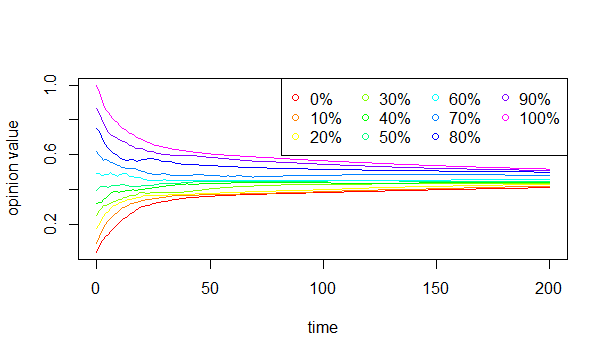
\includegraphics[width=\textwidth]{plots/max-values/spatial-maxv.png}
      \caption[]%
      {{\small Priestorový graf}}    
      \label{fig:prubeh-prostorovy}
  \end{subfigure}
  \vskip\baselineskip
  \begin{subfigure}[b]{0.475\textwidth}   
      \centering 
      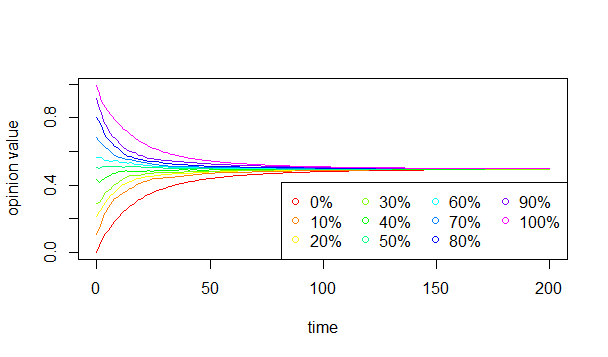
\includegraphics[width=\textwidth]{plots/max-values/small-world-maxv.png}
      \caption[]%
      {{\small Malý svet}}    
      \label{fig:prubeh-maly svet}
  \end{subfigure}
  \quad
  \begin{subfigure}[b]{0.475\textwidth}   
      \centering 
      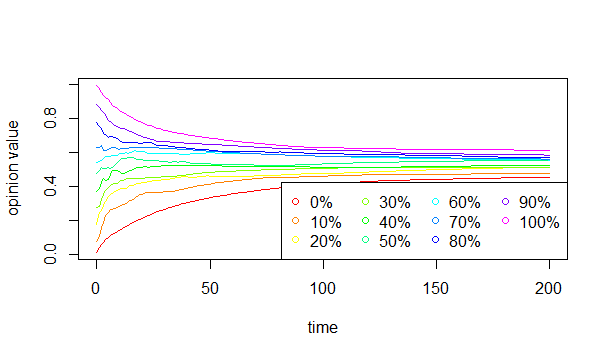
\includegraphics[width=\textwidth]{plots/max-values/prefferentialMaxV.png}
      \caption[]%
      {{\small Preferenčný graf}}    
      \label{fig:prubeh-preferencni}
  \end{subfigure}
  \caption[]
  {\small Vývin hodnot názorů pro jednotlivé grafy}
  \label{fig:prubeh-grafy}
\end{figure*}
 
\chapter{Závěr}
K formování názorů jsme zvolily přístup postupného přizpůsobování se okolí každým z agentů současně. Navrhly jsme model, ve kterém jsou agenti uspořádání v určité topologii a vzájemně interagují, pokud jsou spojeni vazbou. Uvažovaly jsme různé topologie sítí, strategie přebírání názorů i rychlost, s jakou agenti mění názor. I přes množství parametrů však simulace neukázaly výrazný rozdíl v chování modelu. Později jsme přidaly možnost různého počátečního rozdělení hodnot názorů.

Žádný z parametrů výrazně neovlivnil výsledný názor po ustálení změn. Největší dopad měly jednotlivé parametry na rychlost konvergence ke společné shodě. Proto jsme namísto hodnot názorů zkoumaly rychlost vývoje. Velký počet parametrů nám však znemožnil podrobnější analýzu méně výrazných jevů v krátkodobém horizontu.

Projekt by se dal rozšířit dvěma způsoby. První možností je udělat podrobnější analýzu a zkoumat percentuální zastoupení jednotlivých intervalů hodnot v průběhu simulace, výslednou hodnotu názorů a další charakteristiky. Druhou možností je upravit model. Zajímavým obohacením by bylo přidání agentů, jejichž názor se v průběhu simulace nemění, ale pouze ovlivňuje okolí. Tito agenti by znemožnili všeobecnou shodu a model by se choval o poznání dynamičtěji. Dalším obohacením modelu může být pravděpodobnost změny názoru, což by zamezilo okamžité snaze přiblížit se názorem okolí. Tento parametr by však pouze ovlivnil rychlost konvergence. Oba zmíněné parametry jsou v modelu obsaženy, ale v analýze jsme s nimi nepracovaly.

Vytvořily jsme model formování spojitého názoru. Přes větší množství parametrů se model chová velmi stejnorodě a konverguje k přibližně stejné hodnotě. Na druhou stranu nám tyto parametry ztížily analýzu. Nakonec jsme navrhly rozšíření, které by náš model mohly zajímavě obohatit a více přiblížit skutečnosti.

% K formovaniu názorov sme zvolili prístup postupného preberania názorov okolia každým agentom simultánne. Agenti sú usporiadaní v určitej typológii, kde vrcholmi sú ľudia a hranami väzby medzi nimi. Agenti môžu zistiť len názor svojich susedov, s ktorými sú prepojený hranou. 

% Celkovo sme vybrali 4 typy grafov - referenčný, náhodný, priestorový a tzv. malý svet. Preberanie názoru prebieha buď na základe jedného náhodného suseda alebo celého okolia, pričom miera prebratia názoru je taktiež parametrizovaná. Napriek rôznorodosti grafovej štruktúre a dvom typom stratégie preberania názorov, simulácie neukázali výrazný rozdiel v správaní modelu. Pridali sme ďalší parameter - počiatočné rozdelenie hodnôt názorov.

% Žiaden z parametrov výrazne neovplyvnil výsledný názor po ustálení zmien. Najväčší dopad mali jednotlivé parametre na rýchlosť konvergencie k dohode. Preto sme namiesto hodnôt názorov skúmali rýchlosť vývoja. Veľký počet parametrov nám však znemožnil podrobnejšiu analýzu menej výrazných javov v krátkodobom horizonte.

% Projekt by sa dal rozšíriť dvoma spôsobmi, už spomínanou podrobnejšou analýzou (či už percentuálneho zastúpenia jednotlivých intervalov hodnôt počas vývoja, záverečnej hodnoty alebo inej charakteristiky) a samotným modelom. Pre zvýšenie realistickosti by bolo možné do modelu doplniť ľudí s nemenným názorom, ktorí by však ovplyvňovali okolie. Títo ľudia by znemožnili všeobecnú zhodu a model by sa správal podstatne dynamickejšie. Ďalším vylepšením môže byť pravdepodobnosť zmeny názoru, čo by zamedzilo okamžitej snahe priblížiť sa názorom okoliu agentom. V prípade tohto parametru by však možno išlo len o ďalšie ovplyvňovania rýchlosti konvergencie. Oba parametre sú obsiahnuté v momentálnom modele ale v analýze sme na ne nebrali ohľad.

% Vytvorili sme model formovania spojitého názoru. Napriek väčšiemu množstvu parametrov sa model správa rovnorodo a konverguje k približne rovnakej hodnote. Tieto parametre nám na druhú stranu znáročnili analýzu. Nakoniec sme navrhli rozšírenia, ktoré by mohli model viac priblížiť skutočnosti a zároveň by ho mohli spraviť zaujímavejším.
\end{document}